\section{Results and Discussion}
\subsection{Four-Arm Comparison}
Table~\ref{tab:focused_scores} gives both scores and seed dispersion for every arm, family and surface. Fig.~\ref{fig:focused_contrasts} shows all primary and secondary AP contrasts; the companion retains all 36 AP and Hit@3 contrast intervals and all 72 seed-level score rows. The estimates are exploratory comparisons of independently tuned feature pipelines on a previously examined test set.

\begin{table*}[!t]
\caption{Four-arm test scores across the three fitted seeds}
\label{tab:focused_scores}
\centering
\begin{tabular}{lllcc}
\hline
Surface & Family & Arm & AP & Hit@3 \\
\hline
Turf & XGBoost & H & 0.4710 $\pm$ 0.0006 & 0.4580 $\pm$ 0.0004 \\
Turf & XGBoost & $G_{\mathrm{mixed}}$ & 0.4631 $\pm$ 0.0010 & 0.4600 $\pm$ 0.0007 \\
Turf & XGBoost & $G_{\mathrm{ancestor}}$ & 0.4621 $\pm$ 0.0002 & 0.4603 $\pm$ 0.0019 \\
Turf & XGBoost & P & 0.4705 $\pm$ 0.0002 & 0.4621 $\pm$ 0.0015 \\
Turf & LightGBM & H & 0.4738 $\pm$ 0.0005 & 0.4585 $\pm$ 0.0010 \\
Turf & LightGBM & $G_{\mathrm{mixed}}$ & 0.4663 $\pm$ 0.0004 & 0.4645 $\pm$ 0.0006 \\
Turf & LightGBM & $G_{\mathrm{ancestor}}$ & 0.4664 $\pm$ 0.0010 & 0.4629 $\pm$ 0.0015 \\
Turf & LightGBM & P & 0.4736 $\pm$ 0.0002 & 0.4646 $\pm$ 0.0021 \\
Turf & CatBoost & H & 0.4725 $\pm$ 0.0005 & 0.4601 $\pm$ 0.0005 \\
Turf & CatBoost & $G_{\mathrm{mixed}}$ & 0.4668 $\pm$ 0.0002 & 0.4627 $\pm$ 0.0011 \\
Turf & CatBoost & $G_{\mathrm{ancestor}}$ & 0.4667 $\pm$ 0.0006 & 0.4638 $\pm$ 0.0042 \\
Turf & CatBoost & P & 0.4712 $\pm$ 0.0001 & 0.4627 $\pm$ 0.0016 \\
Dirt & XGBoost & H & 0.4561 $\pm$ 0.0007 & 0.4634 $\pm$ 0.0012 \\
Dirt & XGBoost & $G_{\mathrm{mixed}}$ & 0.4541 $\pm$ 0.0009 & 0.4616 $\pm$ 0.0008 \\
Dirt & XGBoost & $G_{\mathrm{ancestor}}$ & 0.4552 $\pm$ 0.0007 & 0.4634 $\pm$ 0.0013 \\
Dirt & XGBoost & P & 0.4575 $\pm$ 0.0009 & 0.4654 $\pm$ 0.0020 \\
Dirt & LightGBM & H & 0.4585 $\pm$ 0.0006 & 0.4650 $\pm$ 0.0013 \\
Dirt & LightGBM & $G_{\mathrm{mixed}}$ & 0.4567 $\pm$ 0.0010 & 0.4614 $\pm$ 0.0020 \\
Dirt & LightGBM & $G_{\mathrm{ancestor}}$ & 0.4578 $\pm$ 0.0004 & 0.4632 $\pm$ 0.0019 \\
Dirt & LightGBM & P & 0.4606 $\pm$ 0.0006 & 0.4680 $\pm$ 0.0023 \\
Dirt & CatBoost & H & 0.4523 $\pm$ 0.0004 & 0.4603 $\pm$ 0.0014 \\
Dirt & CatBoost & $G_{\mathrm{mixed}}$ & 0.4525 $\pm$ 0.0011 & 0.4619 $\pm$ 0.0020 \\
Dirt & CatBoost & $G_{\mathrm{ancestor}}$ & 0.4544 $\pm$ 0.0009 & 0.4644 $\pm$ 0.0011 \\
Dirt & CatBoost & P & 0.4553 $\pm$ 0.0015 & 0.4643 $\pm$ 0.0018 \\
\hline
\end{tabular}
\par\smallskip Scores are fractions, shown as mean $\pm$ sample SD across three paired seeds. The test was previously examined. Cohort denominators are in Table~\ref{tab:cohort}; graph coverage and parent-summary availability are in Table~\ref{tab:focused_coverage}.
\end{table*}

\begin{figure}[!t]
\centering
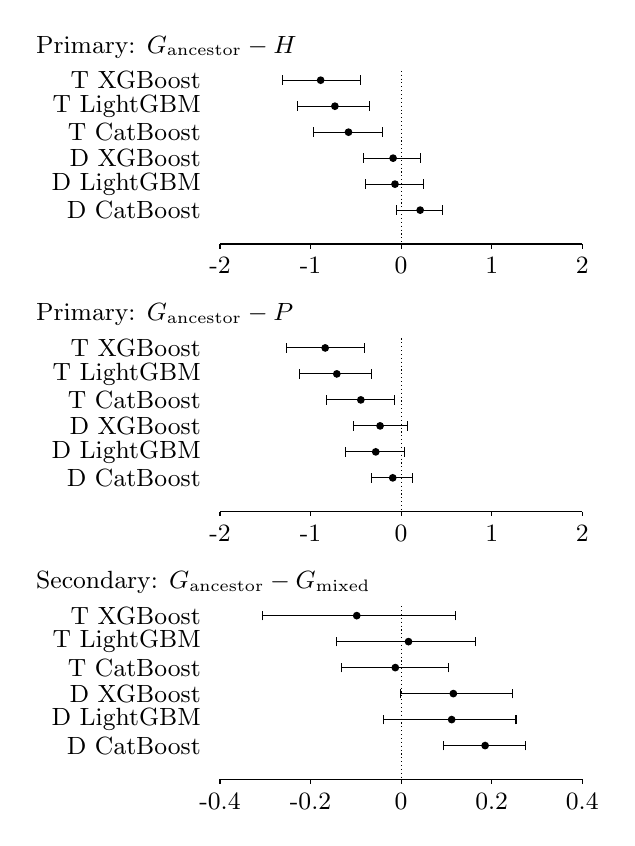
\begin{tikzpicture}[x=1cm,y=1cm]
\small
\node[anchor=west] at (0,-0.000) {Primary: $G_{\mathrm{ancestor}}-H$};
\node[anchor=east] at (2.32,-0.420) {T XGBoost};
\draw (3.2385,-0.420) -- (4.2323,-0.420);
\draw (3.2385,-0.480) -- (3.2385,-0.360);
\draw (4.2323,-0.480) -- (4.2323,-0.360);
\fill (3.7279,-0.420) circle (1.4pt);
\node[anchor=east] at (2.32,-0.750) {T LightGBM};
\draw (3.4320,-0.750) -- (4.3469,-0.750);
\draw (3.4320,-0.810) -- (3.4320,-0.690);
\draw (4.3469,-0.810) -- (4.3469,-0.690);
\fill (3.9088,-0.750) circle (1.4pt);
\node[anchor=east] at (2.32,-1.080) {T CatBoost};
\draw (3.6377,-1.080) -- (4.5131,-1.080);
\draw (3.6377,-1.140) -- (3.6377,-1.020);
\draw (4.5131,-1.140) -- (4.5131,-1.020);
\fill (4.0813,-1.080) circle (1.4pt);
\node[anchor=east] at (2.32,-1.410) {D XGBoost};
\draw (4.2665,-1.410) -- (4.9967,-1.410);
\draw (4.2665,-1.470) -- (4.2665,-1.350);
\draw (4.9967,-1.470) -- (4.9967,-1.350);
\fill (4.6478,-1.410) circle (1.4pt);
\node[anchor=east] at (2.32,-1.740) {D LightGBM};
\draw (4.2961,-1.740) -- (5.0390,-1.740);
\draw (4.2961,-1.800) -- (4.2961,-1.680);
\draw (5.0390,-1.800) -- (5.0390,-1.680);
\fill (4.6719,-1.740) circle (1.4pt);
\node[anchor=east] at (2.32,-2.070) {D CatBoost};
\draw (4.6866,-2.070) -- (5.2736,-2.070);
\draw (4.6866,-2.130) -- (4.6866,-2.010);
\draw (5.2736,-2.130) -- (5.2736,-2.010);
\fill (4.9917,-2.070) circle (1.4pt);
\draw[densely dotted] (4.7500,-0.300) -- (4.7500,-2.500);
\draw (2.45,-2.500) -- (7.05,-2.500);
\draw (2.4500,-2.500) -- (2.4500,-2.560) node[below] {-2};
\draw (3.6000,-2.500) -- (3.6000,-2.560) node[below] {-1};
\draw (4.7500,-2.500) -- (4.7500,-2.560) node[below] {0};
\draw (5.9000,-2.500) -- (5.9000,-2.560) node[below] {1};
\draw (7.0500,-2.500) -- (7.0500,-2.560) node[below] {2};
\node[anchor=west] at (0,-3.400) {Primary: $G_{\mathrm{ancestor}}-P$};
\node[anchor=east] at (2.32,-3.820) {T XGBoost};
\draw (3.2982,-3.820) -- (4.2878,-3.820);
\draw (3.2982,-3.880) -- (3.2982,-3.760);
\draw (4.2878,-3.880) -- (4.2878,-3.760);
\fill (3.7857,-3.820) circle (1.4pt);
\node[anchor=east] at (2.32,-4.150) {T LightGBM};
\draw (3.4620,-4.150) -- (4.3758,-4.150);
\draw (3.4620,-4.210) -- (3.4620,-4.090);
\draw (4.3758,-4.210) -- (4.3758,-4.090);
\fill (3.9330,-4.150) circle (1.4pt);
\node[anchor=east] at (2.32,-4.480) {T CatBoost};
\draw (3.7965,-4.480) -- (4.6691,-4.480);
\draw (3.7965,-4.540) -- (3.7965,-4.420);
\draw (4.6691,-4.540) -- (4.6691,-4.420);
\fill (4.2381,-4.480) circle (1.4pt);
\node[anchor=east] at (2.32,-4.810) {D XGBoost};
\draw (4.1407,-4.810) -- (4.8299,-4.810);
\draw (4.1407,-4.870) -- (4.1407,-4.750);
\draw (4.8299,-4.870) -- (4.8299,-4.750);
\fill (4.4825,-4.810) circle (1.4pt);
\node[anchor=east] at (2.32,-5.140) {D LightGBM};
\draw (4.0443,-5.140) -- (4.7953,-5.140);
\draw (4.0443,-5.200) -- (4.0443,-5.080);
\draw (4.7953,-5.200) -- (4.7953,-5.080);
\fill (4.4275,-5.140) circle (1.4pt);
\node[anchor=east] at (2.32,-5.470) {D CatBoost};
\draw (4.3784,-5.470) -- (4.8995,-5.470);
\draw (4.3784,-5.530) -- (4.3784,-5.410);
\draw (4.8995,-5.530) -- (4.8995,-5.410);
\fill (4.6434,-5.470) circle (1.4pt);
\draw[densely dotted] (4.7500,-3.700) -- (4.7500,-5.900);
\draw (2.45,-5.900) -- (7.05,-5.900);
\draw (2.4500,-5.900) -- (2.4500,-5.960) node[below] {-2};
\draw (3.6000,-5.900) -- (3.6000,-5.960) node[below] {-1};
\draw (4.7500,-5.900) -- (4.7500,-5.960) node[below] {0};
\draw (5.9000,-5.900) -- (5.9000,-5.960) node[below] {1};
\draw (7.0500,-5.900) -- (7.0500,-5.960) node[below] {2};
\node[anchor=west] at (0,-6.800) {Secondary: $G_{\mathrm{ancestor}}-G_{\mathrm{mixed}}$};
\node[anchor=east] at (2.32,-7.220) {T XGBoost};
\draw (2.9845,-7.220) -- (5.4389,-7.220);
\draw (2.9845,-7.280) -- (2.9845,-7.160);
\draw (5.4389,-7.280) -- (5.4389,-7.160);
\fill (4.1863,-7.220) circle (1.4pt);
\node[anchor=east] at (2.32,-7.550) {T LightGBM};
\draw (3.9301,-7.550) -- (5.6971,-7.550);
\draw (3.9301,-7.610) -- (3.9301,-7.490);
\draw (5.6971,-7.610) -- (5.6971,-7.490);
\fill (4.8436,-7.550) circle (1.4pt);
\node[anchor=east] at (2.32,-7.880) {T CatBoost};
\draw (3.9932,-7.880) -- (5.3536,-7.880);
\draw (3.9932,-7.940) -- (3.9932,-7.820);
\draw (5.3536,-7.940) -- (5.3536,-7.820);
\fill (4.6762,-7.880) circle (1.4pt);
\node[anchor=east] at (2.32,-8.210) {D XGBoost};
\draw (4.7390,-8.210) -- (6.1605,-8.210);
\draw (4.7390,-8.270) -- (4.7390,-8.150);
\draw (6.1605,-8.270) -- (6.1605,-8.150);
\fill (5.4131,-8.210) circle (1.4pt);
\node[anchor=east] at (2.32,-8.540) {D LightGBM};
\draw (4.5229,-8.540) -- (6.2089,-8.540);
\draw (4.5229,-8.600) -- (4.5229,-8.480);
\draw (6.2089,-8.600) -- (6.2089,-8.480);
\fill (5.3916,-8.540) circle (1.4pt);
\node[anchor=east] at (2.32,-8.870) {D CatBoost};
\draw (5.2924,-8.870) -- (6.3288,-8.870);
\draw (5.2924,-8.930) -- (5.2924,-8.810);
\draw (6.3288,-8.930) -- (6.3288,-8.810);
\fill (5.8166,-8.870) circle (1.4pt);
\draw[densely dotted] (4.7500,-7.100) -- (4.7500,-9.300);
\draw (2.45,-9.300) -- (7.05,-9.300);
\draw (2.4500,-9.300) -- (2.4500,-9.360) node[below] {-0.4};
\draw (3.6000,-9.300) -- (3.6000,-9.360) node[below] {-0.2};
\draw (4.7500,-9.300) -- (4.7500,-9.360) node[below] {0};
\draw (5.9000,-9.300) -- (5.9000,-9.360) node[below] {0.2};
\draw (7.0500,-9.300) -- (7.0500,-9.360) node[below] {0.4};
\end{tikzpicture}
\caption{All prespecified AP differences, in percentage points (100 times the fraction difference). T and D denote turf and dirt. Points average paired seed-specific differences; whiskers are descriptive 95\% paired whole-race bootstrap percentile intervals, conditional on the fitted models and unadjusted for multiple comparisons. Panels use their indicated scales. The test was previously examined. Denominators and coverage are in Tables~\ref{tab:cohort} and \ref{tab:focused_coverage}.}
\label{fig:focused_contrasts}
\end{figure}


On turf, $G_{\mathrm{ancestor}}$--H AP differences are $-0.0089$, $-0.0073$ and $-0.0058$ for XGBoost, LightGBM and CatBoost; the corresponding $G_{\mathrm{ancestor}}$--P differences are $-0.0084$, $-0.0071$ and $-0.0045$. All six descriptive paired intervals lie below zero. On dirt, all six primary AP intervals include zero. All 12 primary Hit@3 intervals include zero. Thus the tested ancestor-rule graph group does not establish a consistent AP benefit over H or P across families and surfaces; intervals containing zero do not establish equivalence.

The secondary $G_{\mathrm{ancestor}}$--$G_{\mathrm{mixed}}$ contrast for CatBoost on dirt is $+0.0019$ AP with interval $[0.0009,0.0027]$, and $+0.0026$ Hit@3 with interval $[0.0002,0.0048]$. The other secondary AP intervals include zero. This exploratory comparison concerns whole independently tuned pipelines and does not isolate fallback or demonstrate improvement over H or P.

\subsection{Coverage and Parent-Feature Availability}
All $G_{\mathrm{ancestor}}$ training entries resolve at depth 1; some validation and test entries require deeper ancestors (Table~\ref{tab:focused_coverage}). No entry has a missing graph representation in the audited views. For $G_{\mathrm{mixed}}$, direct vectors cover all training entries but only 12.97\% of turf and 12.06\% of dirt test entries. All test entries have the three parent identifiers, but a known parent need not have a qualifying prior same-surface start: sire/dam/damsire zero-prior rates are 30.14\%/41.27\%/4.56\% on turf and 28.87\%/43.86\%/5.19\% on dirt. These entry-weighted rates differ from unseen categorical-parent rates in the historical B pipeline. Same-rule construction does not eliminate this coverage or cohort shift.

\begin{figure}[!t]
\centering
% Column-width layout; all coordinates come from the frozen aggregate CSV.
% Source SHA-256: 17520174da8f6867a9afb1de974d1ad441bd3ad7eb8069bdf0c2724603b47e44
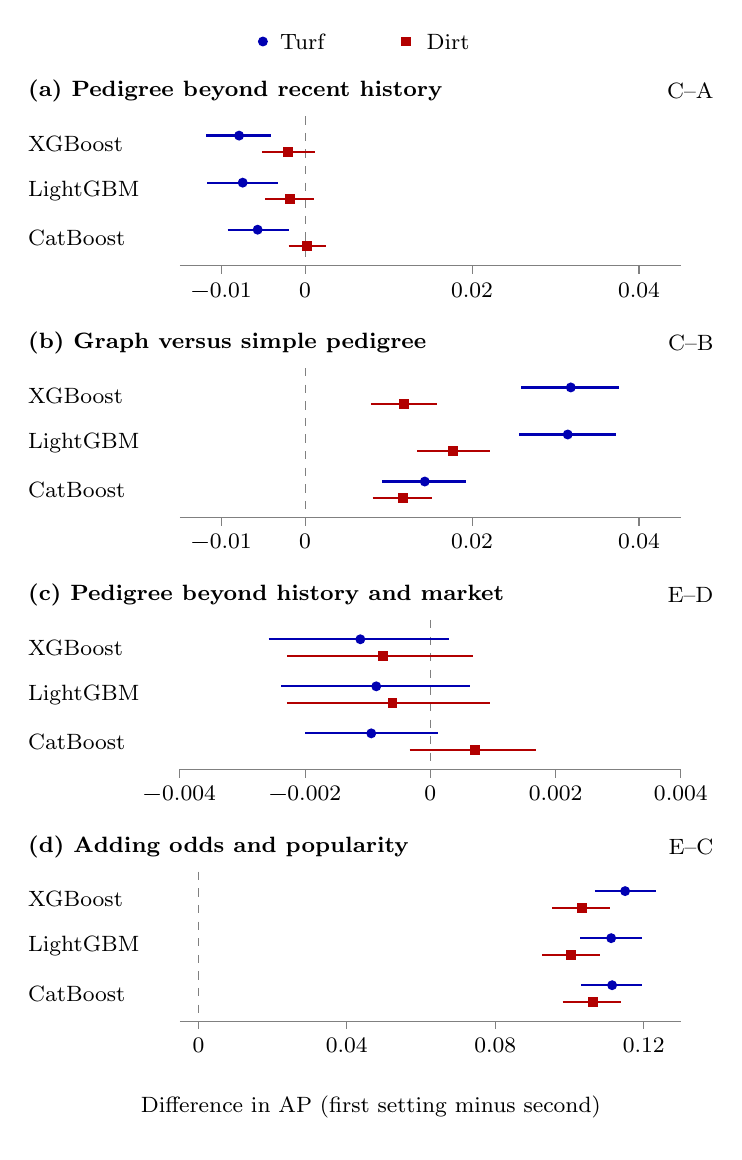
\begin{tikzpicture}[x=1pt,y=1pt,every node/.style={font=\footnotesize,inner sep=0pt}]
\useasboundingbox (0,-376) rectangle (248,23);
\fill[blue!70!black] (85,18) circle (1.8pt);
\node[anchor=west] at (91,18) {Turf};
\fill[red!70!black] (135,16.2) rectangle (138.6,19.8);
\node[anchor=west] at (144,18) {Dirt};
\node[anchor=west,font=\footnotesize\bfseries] at (0,0) {(a) Pedigree beyond recent history};
\node[anchor=east] at (248,0) {C--A};
\draw[gray,dashed] (100.25000,-9) -- (100.25000,-63);
\node[anchor=west] at (0,-19.0) {XGBoost};
\draw[blue!70!black,line width=0.8pt] (64.51879,-16) -- (88.08954,-16);
\fill[blue!70!black] (76.39434,-16) circle (1.8pt);
\draw[red!70!black,line width=0.8pt] (84.64982,-22) -- (103.72371,-22);
\fill[red!70!black] (92.28964,-23.8) rectangle (95.88964,-20.2);
\node[anchor=west] at (0,-36.0) {LightGBM};
\draw[blue!70!black,line width=0.8pt] (64.96685,-33) -- (90.31166,-33);
\fill[blue!70!black] (77.69231,-33) circle (1.8pt);
\draw[red!70!black,line width=0.8pt] (85.85195,-39) -- (103.52991,-39);
\fill[red!70!black] (93.03398,-40.8) rectangle (96.63398,-37.2);
\node[anchor=west] at (0,-53.0) {CatBoost};
\draw[blue!70!black,line width=0.8pt] (72.26109,-50) -- (94.30283,-50);
\fill[blue!70!black] (83.09692,-50) circle (1.8pt);
\draw[red!70!black,line width=0.8pt] (94.30643,-56) -- (107.76023,-56);
\fill[red!70!black] (99.19380,-57.8) rectangle (102.79380,-54.2);
\draw[gray] (55,-63) -- (236,-63);
\draw[gray] (70.08333,-63) -- (70.08333,-66);
\node[anchor=north] at (70.08333,-69) {\textminus{}0.01};
\draw[gray] (100.25000,-63) -- (100.25000,-66);
\node[anchor=north] at (100.25000,-69) {0};
\draw[gray] (160.58333,-63) -- (160.58333,-66);
\node[anchor=north] at (160.58333,-69) {0.02};
\draw[gray] (220.91667,-63) -- (220.91667,-66);
\node[anchor=north] at (220.91667,-69) {0.04};
\node[anchor=west,font=\footnotesize\bfseries] at (0,-91) {(b) Graph versus simple pedigree};
\node[anchor=east] at (248,-91) {C--B};
\draw[gray,dashed] (100.25000,-100) -- (100.25000,-154);
\node[anchor=west] at (0,-110.0) {XGBoost};
\draw[blue!70!black,line width=0.8pt] (178.40832,-107) -- (213.83245,-107);
\fill[blue!70!black] (196.25532,-107) circle (1.8pt);
\draw[red!70!black,line width=0.8pt] (124.01340,-113) -- (147.95615,-113);
\fill[red!70!black] (134.19110,-114.8) rectangle (137.79110,-111.2);
\node[anchor=west] at (0,-127.0) {LightGBM};
\draw[blue!70!black,line width=0.8pt] (177.59525,-124) -- (212.46516,-124);
\fill[blue!70!black] (195.14491,-124) circle (1.8pt);
\draw[red!70!black,line width=0.8pt] (140.74645,-130) -- (166.89437,-130);
\fill[red!70!black] (151.95101,-131.8) rectangle (155.55101,-128.2);
\node[anchor=west] at (0,-144.0) {CatBoost};
\draw[blue!70!black,line width=0.8pt] (128.06113,-141) -- (158.35925,-141);
\fill[blue!70!black] (143.49464,-141) circle (1.8pt);
\draw[red!70!black,line width=0.8pt] (124.62271,-147) -- (146.03829,-147);
\fill[red!70!black] (133.80366,-148.8) rectangle (137.40366,-145.2);
\draw[gray] (55,-154) -- (236,-154);
\draw[gray] (70.08333,-154) -- (70.08333,-157);
\node[anchor=north] at (70.08333,-160) {\textminus{}0.01};
\draw[gray] (100.25000,-154) -- (100.25000,-157);
\node[anchor=north] at (100.25000,-160) {0};
\draw[gray] (160.58333,-154) -- (160.58333,-157);
\node[anchor=north] at (160.58333,-160) {0.02};
\draw[gray] (220.91667,-154) -- (220.91667,-157);
\node[anchor=north] at (220.91667,-160) {0.04};
\node[anchor=west,font=\footnotesize\bfseries] at (0,-182) {(c) Pedigree beyond history and market};
\node[anchor=east] at (248,-182) {E--D};
\draw[gray,dashed] (145.50000,-191) -- (145.50000,-245);
\node[anchor=west] at (0,-201.0) {XGBoost};
\draw[blue!70!black,line width=0.8pt] (87.03301,-198) -- (152.25539,-198);
\fill[blue!70!black] (120.20592,-198) circle (1.8pt);
\draw[red!70!black,line width=0.8pt] (93.71246,-204) -- (160.80955,-204);
\fill[red!70!black] (126.46760,-205.8) rectangle (130.06760,-202.2);
\node[anchor=west] at (0,-218.0) {LightGBM};
\draw[blue!70!black,line width=0.8pt] (91.60293,-215) -- (159.96085,-215);
\fill[blue!70!black] (125.96019,-215) circle (1.8pt);
\draw[red!70!black,line width=0.8pt] (93.69963,-221) -- (167.05269,-221);
\fill[red!70!black] (130.02503,-222.8) rectangle (133.62503,-219.2);
\node[anchor=west] at (0,-235.0) {CatBoost};
\draw[blue!70!black,line width=0.8pt] (100.28261,-232) -- (148.36689,-232);
\fill[blue!70!black] (124.15522,-232) circle (1.8pt);
\draw[red!70!black,line width=0.8pt] (138.00584,-238) -- (183.73966,-238);
\fill[red!70!black] (159.73706,-239.8) rectangle (163.33706,-236.2);
\draw[gray] (55,-245) -- (236,-245);
\draw[gray] (55.00000,-245) -- (55.00000,-248);
\node[anchor=north] at (55.00000,-251) {\textminus{}0.004};
\draw[gray] (100.25000,-245) -- (100.25000,-248);
\node[anchor=north] at (100.25000,-251) {\textminus{}0.002};
\draw[gray] (145.50000,-245) -- (145.50000,-248);
\node[anchor=north] at (145.50000,-251) {0};
\draw[gray] (190.75000,-245) -- (190.75000,-248);
\node[anchor=north] at (190.75000,-251) {0.002};
\draw[gray] (236.00000,-245) -- (236.00000,-248);
\node[anchor=north] at (236.00000,-251) {0.004};
\node[anchor=west,font=\footnotesize\bfseries] at (0,-273) {(d) Adding odds and popularity};
\node[anchor=east] at (248,-273) {E--C};
\draw[gray,dashed] (61.70370,-282) -- (61.70370,-336);
\node[anchor=west] at (0,-292.0) {XGBoost};
\draw[blue!70!black,line width=0.8pt] (204.98782,-289) -- (227.01629,-289);
\fill[blue!70!black] (215.88242,-289) circle (1.8pt);
\draw[red!70!black,line width=0.8pt] (189.56320,-295) -- (210.43406,-295);
\fill[red!70!black] (198.48559,-296.8) rectangle (202.08559,-293.2);
\node[anchor=west] at (0,-309.0) {LightGBM};
\draw[blue!70!black,line width=0.8pt] (199.64401,-306) -- (221.82729,-306);
\fill[blue!70!black] (210.84720,-306) circle (1.8pt);
\draw[red!70!black,line width=0.8pt] (185.94791,-312) -- (206.65524,-312);
\fill[red!70!black] (194.53162,-313.8) rectangle (198.13162,-310.2);
\node[anchor=west] at (0,-326.0) {CatBoost};
\draw[blue!70!black,line width=0.8pt] (200.02759,-323) -- (222.14920,-323);
\fill[blue!70!black] (211.18912,-323) circle (1.8pt);
\draw[red!70!black,line width=0.8pt] (193.31513,-329) -- (214.43024,-329);
\fill[red!70!black] (202.58211,-330.8) rectangle (206.18211,-327.2);
\draw[gray] (55,-336) -- (236,-336);
\draw[gray] (61.70370,-336) -- (61.70370,-339);
\node[anchor=north] at (61.70370,-342) {0};
\draw[gray] (115.33333,-336) -- (115.33333,-339);
\node[anchor=north] at (115.33333,-342) {0.04};
\draw[gray] (168.96296,-336) -- (168.96296,-339);
\node[anchor=north] at (168.96296,-342) {0.08};
\draw[gray] (222.59259,-336) -- (222.59259,-339);
\node[anchor=north] at (222.59259,-342) {0.12};
\node at (124,-367) {Difference in AP (first setting minus second)};
\end{tikzpicture}

\caption{Historical AP contrasts. Positive values favor the first setting. Points average paired seed differences; bars are descriptive 95\% whole-race bootstrap intervals, conditional on fitted models and unadjusted for multiplicity. Panels (a)--(b) share a scale; others differ. Market fields are retrospective and absent from the new arms.}
\label{fig:historical_contrasts}
\end{figure}

\subsection{Historical Market and Parent-ID Context}
\begin{table*}[!t]
\caption{Historical Market-Information Scores Across All Families and Surfaces}
\label{tab:historical_market}
\centering
\begin{tabular}{llrrrrrr}
\hline
& & \multicolumn{3}{c}{Entry AP} & \multicolumn{3}{c}{Mean Hit@3} \\
Family & Surface & D & E & F & D & E & F \\
\hline
XGBoost & Turf & 0.5792 & 0.5781 & 0.5679 & 0.5400 & 0.5382 & 0.5363 \\
XGBoost & Dirt & 0.5582 & 0.5574 & 0.5507 & 0.5285 & 0.5287 & 0.5261 \\
LightGBM & Turf & 0.5784 & 0.5775 & 0.5668 & 0.5387 & 0.5386 & 0.5360 \\
LightGBM & Dirt & 0.5577 & 0.5571 & 0.5496 & 0.5291 & 0.5283 & 0.5269 \\
CatBoost & Turf & 0.5793 & 0.5783 & 0.5676 & 0.5395 & 0.5380 & 0.5365 \\
CatBoost & Dirt & 0.5582 & 0.5589 & 0.5511 & 0.5286 & 0.5275 & 0.5265 \\
\hline
\end{tabular}
\par\smallskip Historical three-seed means: D adds final odds and popularity to history; E adds them to the original graph pipeline; F uses final odds alone. The market fields are retrospective and are not inputs in the new four-arm study.
\end{table*}

Table~\ref{tab:historical_market} retains every family and surface for the earlier market-informed settings; Fig.~\ref{fig:historical_contrasts} retains all four historical AP contrasts. Odds alone gives AP 0.5668--0.5679 on turf and 0.5496--0.5511 on dirt. In the historical E--D comparison, all six AP intervals include zero. Adding final odds and popularity to C (E--C) increases AP by approximately 0.1004--0.1150 and Hit@3 by 0.066--0.078. These are independently tuned comparisons with retrospective final-market inputs, not isolated causal effects or evidence of betting profit. They do not test the new $G_{\mathrm{ancestor}}$ or P arms with market features.





Historically, C outperformed the tested categorical-parent B pipeline, but B was weaker than A; this does not establish added value beyond history or superiority over the supervised P comparator. Test sire/dam identifiers were unseen in the historical training-surface vocabulary for 30.04\%/38.73\% of turf entries and 28.75\%/42.15\% of dirt entries. The earlier no-observed-history subgroup was added after test release and is not necessarily a true debut cohort. The corrected deterministic random baseline has Hit@3 of 0.2431 turf and 0.2161 dirt, against analytical expectations 0.2433 and 0.2188.

\subsection{Interpretation and Limitations}
The contrasts concern the specified independently tuned pipelines and their feature groups. They do not measure a causal effect of pedigree, isolate fallback from all other representation differences, or establish whether a different graph architecture or ancestry model would help. A common ancestor construction rule does not equate coverage or distributions across partitions. The graph retains the influence of focal horses and later training roots; retrospective pedigree collection does not establish historical record availability. P is a simple supervised comparator with left-censored source history and an increasingly aged frozen map. Its results do not describe an always-updated parent model.

The previously examined test set, unadjusted multiple comparisons and dependence from repeated horses limit inference. Three paired seeds confound graph and classifier randomness; the race bootstrap is conditional on the fitted seeds. The observed collection omits some histories and does not cover all racing jurisdictions. Race-day variables may not have been available at a common prediction horizon, and no dedicated ranker, prospective deployment or betting-profit evaluation is included. These limits constrain transfer and operational claims even if a contrast is favorable.

\section{Conclusion}
In this exploratory same-cohort evaluation, the tested ancestor-rule graph pipeline did not consistently improve AP beyond either recent history or the specified chronological parent-performance pipeline. Turf primary contrasts were negative; dirt intervals included zero. The secondary CatBoost dirt comparison favored the ancestor-rule pipeline over the original mixed pipeline, but does not identify a fallback effect or establish improvement over the primary controls. Historical retrospective market comparisons remain separate and do not evaluate the new four arms beyond market information. Future work requires historically timestamped inputs and an unexamined cohort.

\section*{Data and Code Availability}
Race and pedigree records came from Netkeiba \cite{netkeibaRace,netkeibaDb}. Public data, graph/feature exports, models and predictions are on Kaggle (version 1): \url{https://www.kaggle.com/datasets/charischerw/jra-pedigree-graph-study-2010-2025}. Code, configurations, aggregate results and reproduction instructions are at \url{https://github.com/CharisBerlian/jra-pedigree-graph-study} (release v1.0.5-paper). Data/results use CC BY 4.0; study-authored code uses MIT, with third-party licenses retained. The repository documents environments and limits; independent full-data retraining has not been established.
